\chapter{File Formats}

\section{Executable and Linkable Format (ELF)}

The ELF format is the file format for executable programs on most *NIX systems.

Comes in two formats: 32-bit and 64-bit.

\begin{center}
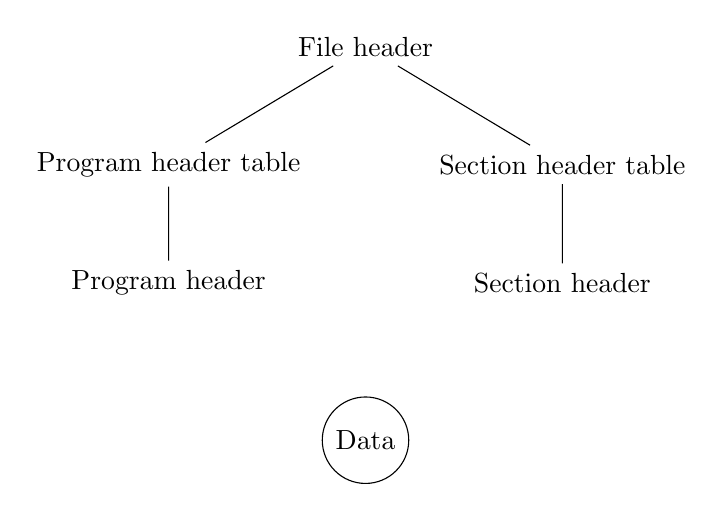
\begin{tikzpicture}[sibling distance=5cm, every node/.style={align=center}]
  \node {File header}
    child { node {Program header table}
      child { node {Program header} }
    }
    child { node {Section header table}
      child { node {Section header} }
    };

  \node [circle, draw] at (0, -5) {Data};
\end{tikzpicture}
\end{center}

\subsection{File header}

The beginning 16 bytes of the file are byte order agnostic.
The first byte must have the value $(7\text{F})_{16}$ (127) followed by
$(45)_{16}$, $(4\text{C})_{16}$, and $(46)_{16}$ (ELF in ASCII encoding).

\subsection{Program header table}

\subsection{Section header table}

This section is only used for linking(?).
